\documentclass[usenames,dvipsnames,mathserif,compress]{beamer}
\usepackage[utf8]{inputenc}
\usepackage[T1]{fontenc}
\usepackage{amsmath}
\usepackage{amssymb}
\usepackage{listings}

\lstset{%,
  basicstyle=\small\ttfamily,
  keywordstyle=\color{red},
  identifierstyle=\color{Blue},
  stringstyle=\color{Green},
  commentstyle=\ttfamily\color{RoyalPurple},
  showstringspaces=false,
  language=C}%,


\author{Ask Hjorth Larsen}
\title{Introduction to high-performance computing}
\institute{Nano-bio Spectroscopy Group and ETSF Scientific Development Centre,\\
Universidad del País Vasco UPV/EHU, San Sebastián, Spain}

\begin{document}
%  hello world

\begin{frame}
  \maketitle
\end{frame}

\begin{frame}
  \begin{block}{The CPU}
    \begin{itemize}
    \item The CPU reads \alert{instructions and inputs}, then performs those instructions on the inputs
    \item Instruction codes and inputs are stored in workspaces
      on the CPU called \alert{registers}
    \item Each cycle, the CPU can execute an instruction; different
      CPU architectures support different instructions
    \end{itemize}
  \end{block}
  \begin{block}{Example}
    \begin{itemize}
    \item Retrieve number from address A, put it in register R
    \item Add numbers from registers R and R', store sum in R''
    \item Write number from R'' to address A'
    \item Etc.
    \end{itemize}
  \end{block}
\end{frame}


\begin{frame}
  \frametitle{Floating point numbers}
  Computational physics mostly boils down to multiplying floating point numbers.
  \begin{block}{IEEE 754 standard for floating point numbers}
    \begin{itemize}
    \item Number is represented as $M \times 2^n$
    \item $M$ is the significand or mantissa
    \item $n$ is the exponent
    \end{itemize}
  \end{block}
  \begin{block}{Important types}
    \begin{itemize}
    \item 32-bit single precision: 24 bit for $M$, 8 for $n$
    \item 64-bit double precision: 53 bit for $M$, 11 for $n$
    \end{itemize}
  \end{block}
  Floating point operations are complex.
  Modern CPUs have one or more \alert{floating point units} (FPUs)
  that execute floating point operations efficiently
\end{frame}


\begin{frame}
  \frametitle{Pipelining}
  \begin{itemize}
  \item Different ``units'' process different parts of multi-step operation
  \item Illustration of pipelining for 4-step operation running 6 times:\\
    \begin{table}
    \begin{tabular}{c|cccccccccccc}
      & u1 &u2&u3&u4\\\hline
      Cycle 1 & A$^1$ &ø&ø&ø \\
      Cycle 2 & B$^1$ & A$^2$ &ø&ø \\
      Cycle 3 & C$^1$ & B$^2$ & A$^3$ &ø \\
      Cycle 4 & D$^1$ & C$^2$ & B$^3$ & A$^4$  \\
      Cycle 5 & E$^1$ & D$^2$ & C$^3$ & B$^4$   \\
      Cycle 6 & F$^1$ & E$^2$ & D$^3$ & C$^4$  \\
      Cycle 7 & ø     & F$^2$ & E$^3$ & D$^4$  \\
      Cycle 8 & ø & ø & F$^3$ & E$^4$  \\
      Cycle 9 & ø & ø & ø & F$^4$  \\
    \end{tabular}
    \end{table}
  \item Clock cycles are wasted while pipeline flushes or fills
  \item Pipelining depends on predictability: Next input element must be readily available
  \end{itemize}
\end{frame}

\begin{frame}
  \frametitle{Branching and pipelining}
  \begin{itemize}
  \item We know that jumping around in memory when retrieving data is bad
  \item Jumping around in the \emph{code} is also bad as it breaks pipelining
  \item Avoid branching in high-performance loops: \texttt{if} statements, function calls, \texttt{goto}, \ldots
  \item Jump can be eliminated by \alert{inlining} --- include the source of a function ``inline'' in place of calling the function, e.g.\ using a macro
  \item Also: \texttt{inline double myfunction(...)}
  \end{itemize}
\end{frame}


\begin{frame}
  \frametitle{Memory and multilevel caching}
  Example: Intel i7-4770 Haswell architecture\\
  \medskip
  \begin{tabular}{llll}
     & Size & Latency & Total \\
    \hline\hline
    L1 cache & 64 KB/core & 4--5 cycles & 1.3 ns\\
    L2 cache & 256 KB/core & 12 cycles & 3.5 ns \\
    L3 cache & 8 MB, shared & 36 cycles & 11 ns\\
    Main memory & 32 GB, shared & $36\textsf{ cycles} + 57$ ns & 68 ns\\\hline\hline
  \end{tabular}
  Source: \url{http://www.7-cpu.com/cpu/Haswell.html}
  \bigskip
  \begin{itemize}
  \item When accessing memory, contiguous chunks of memory will be copied into cache
  \item Cached memory access is very efficient
  \item A failed cache lookup is called a ``cache miss''
  \item Upon cache miss, element is looked up at next (slower) level
  \end{itemize}

\end{frame}



\begin{frame}
  \frametitle{Arrays and memory layout}
  \begin{itemize}
  \item  Standard mathematical matrix notation:
  \begin{align}
    \left[
  \begin{matrix}
    1,1 & 1,2 & 1,3 \\
    2,1 & 2,2 & 2,3 \\
    3,1 & 3,2 & 3,3
  \end{matrix}
  \right]
  \end{align}
\item Elements of the array are stored in a \alert{contiguous} chunk of memory,
  but the ordering depends on language
\item Fortran memory order is \alert{column-major}:
  \begin{tabular}{|c|c|c|c|c|c|c|c|c|}
    \hline
     $1,1$&$2,1$&$3,1$&$1,2$&$2,2$&$3,2$&$1,3$&$2,3$&$3,3$ \\\hline
  \end{tabular}
\item C memory order is \alert{row-major}:
  \begin{tabular}{|c|c|c|c|c|c|c|c|c|}
    \hline
     $1,1$&$1,2$&$1,3$&$2,1$&$2,2$&$2,3$&$3,1$&$3,2$&$3,3$ \\\hline
  \end{tabular}
\item Accessing elements in memory order is fast.
  \end{itemize}
\end{frame}

\begin{frame}[fragile]
  \frametitle{Optimizing cache use}
  \begin{itemize}
  \item Work on contiguous chunks of memory
  \end{itemize}
\begin{lstlisting}
for(i=0; i < N; i++) {
  for(j=0; j < M; j++) {
    a[i * N + j] = ...
  }
}
\end{lstlisting}
vs
\begin{lstlisting}
for(j=0; j < M; j++) {
  for(i=0; i < N; i++) {
    a[i * N + j] = ...
  }
}
\end{lstlisting}
\end{frame}

\begin{frame}[fragile]
  \frametitle{Benchmark}
  \begin{align}
    \hspace{-2cm} \textrm{Matrix multiplication}\quad c_{ij} &= \sum_k a_{ik} b_{kj}\nonumber
  \end{align}
\begin{lstlisting}
void matmul_ikj(int I, int J, int K,
                double *A, double *B, double *C)
{
  int i, j, k;
  for(i=0; i < I; i++) {
    for(k=0; k < K; k++) {
      for(j=0; j < J; j++) {
        C[i * J + j] += A[i * K + k] * B[k * J + j];
      }
    }
  }
}
\end{lstlisting}
Different permutations of $\{ikj\}$ loops will perform differently
\end{frame}


\begin{frame}
  \begin{figure}
  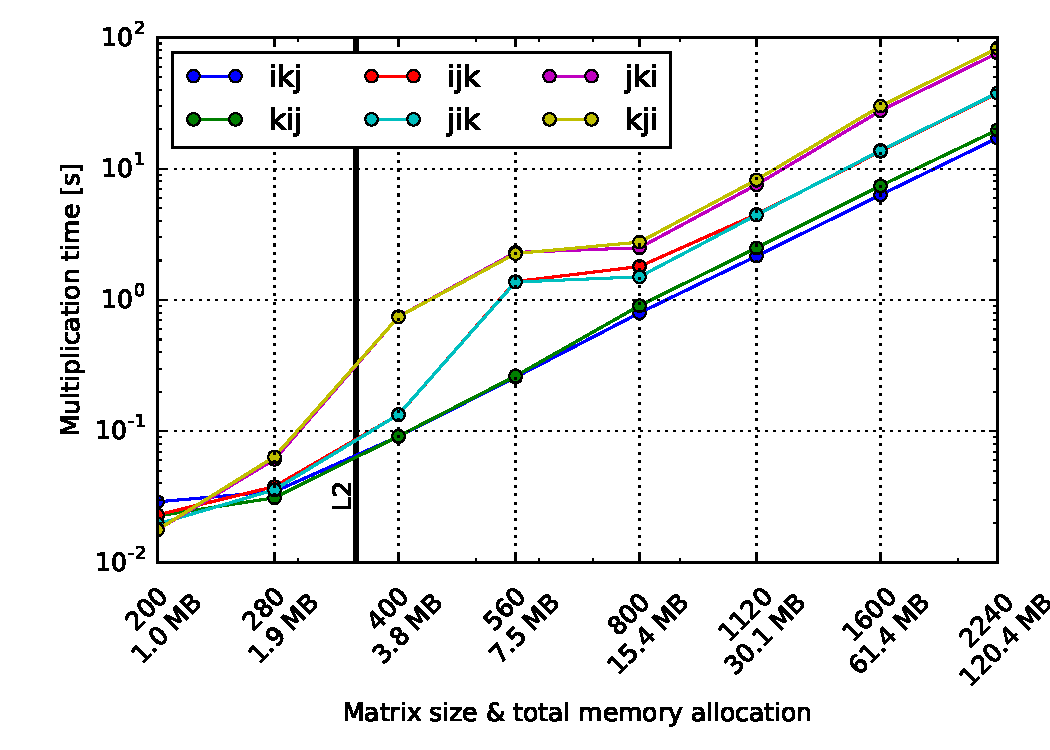
\includegraphics[width=\textwidth]{code/timings-matmul}
  \caption{Timings for matrix multiplication with different loop order
  at \texttt{-O2} optimization level}
  \end{figure}
\end{frame}

% Part 1: HPC
%  * floating point operations
%  * pipelining
%  * cache levels
%  * loop unrolling
%  * matmul
%  * BLAS

\begin{frame}[fragile]
  \frametitle{Loop unrolling}
\begin{lstlisting}
for(i=0; i < 4; i++) {
    a[i] = b[i] * c[i];
}
\end{lstlisting}
vs
\begin{lstlisting}
  a[i] = b[i] * c[i];
  a[i + 1] = b[i + 1] * c[i + 1];
  a[i + 2] = b[i + 2] * c[i + 2];
  a[i + 3] = b[i + 3] * c[i + 3];
\end{lstlisting}
\begin{itemize}
\item Eliminates bounds check on \texttt{i}
\item Compiler may be able to unroll automatically (e.g.~\texttt{-funroll-loops}).
\end{itemize}
\end{frame}

\begin{frame}
  \frametitle{Blocking}
  \begin{itemize}
  \item
  Compute $\mathbf C = \mathbf A \mathbf B$ where each matrix is composed into
  blocks:
  \begin{align}
    \mathbf A = \left[
      \begin{matrix}
        \mathbf A_{11} &\cdots& \mathbf A_{1n}\\
        \vdots & & \vdots \\
        \mathbf A_{n1} & \cdots & \mathbf A_{nn}
      \end{matrix}\right]
  \end{align}

\item Matrix product expressed with blocks:
  \begin{align}
    \mathbf C_{ij} = \sum_{k} \mathbf A_{ik} \mathbf B_{kj}
  \end{align}
  \item Work on smaller blocks that fit into cache
  \item Optimal blocksize depends on architecture (e.g.\ cache size)
  \item Matrix product scales as $\mathcal O(N^3)$
  \item Blocking improves $\mathcal O(N^3)$ prefactor by working on
    chunks that fit in cache
  \end{itemize}
\end{frame}


\begin{frame}
  \frametitle{BLAS}
  \framesubtitle{Basic Linear Algebra Subprograms}
  \begin{itemize}
  \item Standard interface for standard operations:
    Matrix multiplication
  \item Highly optimized for different platforms
  \end{itemize}
  \begin{block}{Some BLAS implementations}
    \begin{itemize}
    \item RefBlas --- reference implementation from Netlib
    \item OpenBlas (based on older GotoBlas)
    \item Atlas --- automatically tuned linear algebra software
    \item Intel MKL
    \item AMD ACML
    \end{itemize}
  \end{block}
\end{frame}

\begin{frame}
  \begin{block}{Some BLAS functions}
    \begin{itemize}
    \item \texttt{dgemm}: \alert double-precision \alert{ge}neral \alert matrix--\alert matrix multiply
    \item \texttt{dsymv}: \alert double-precision \alert{sy}mmetric \alert matrix--\alert vector multiply
    \item \texttt{daxpy}: double-precision $\alert{a \mathbf X}\textrm{ \alert plus } \alert y$
    \item \texttt{zsyr2k}: ``complex double-precision (\alert z) \alert{sy}mmetric \alert ran\alert{k-2} update'',
      $\mathbf X \mathbf Y^T + \mathbf Y \mathbf X^T$
    \item Etc.
    \end{itemize}
  \end{block}
  \begin{block}{LAPACK, Linear Algebra PACKage}
    \begin{itemize}
    \item Higher-level linear algebra operations
    \item LU-decomposition, eigenvalues, \ldots
    \item \texttt{dsyev}: \alert double-precision \alert{sy}mmetric \alert eigen{\alert v}alues
    \item Etc.
    \end{itemize}
  \end{block}
  For best performance, use BLAS/LAPACK whenever possible
\end{frame}

% Part 2: Parallelization
%  * threading
%  * MPI/distributed-memory
%  * Amdahl's law etc.
%  * Discussion of efficiency
%  * Examples?  Redist-calculate-redist
%  * ScaLAPACK

\begin{frame}
  \frametitle{Parallel programs}
  \begin{block}{Shared memory}
    \begin{itemize}
    \item Different threads work at the same time, can have access to same variables
    \item If one process reads while another process writes, bad things happen
    \item Threads must therefore \alert{synchronize} access to the memory
      (e.g.~\texttt{synchronized} methods and blocks in Java)
    \item Lock, run, unlock
    \end{itemize}
  \end{block}
  \begin{block}{Distributed memory}
    \begin{itemize}
    \item Each process has its own chunk of memory, probably on different physical computers
    \item No problem with synchronizing memory (unless also threading)
    \item Must manually send/receive all data
    \end{itemize}
  \end{block}
\end{frame}

\begin{frame}
  \frametitle{Parallel deadlocks}
  \begin{block}{Example}
  \begin{itemize}
  \item Resource A is blocked by process N
  \item Process N waits for resource B
  \item Resource B is blocked by process M
  \item Process M waits for resource A
  %\item Process A expects 10 bytes from process B
  %\item Process B sends only 5 bytes
  %\item Process A holds resource X, waits for resource Y
  %\item Process B holds resource Y, waits for resource X
  \end{itemize}
  \end{block}

  \begin{block}{Example: Distributed memory}
    \begin{itemize}
    \item Process 1 sends 5 numbers to process 2
    \item Process 1 expects something from process 2
    \item Process 2 expects 6 numbers from process 1, receives 5
    \item Both processes wait forever
    \end{itemize}
  \end{block}
\end{frame}

\begin{frame}[fragile]
  \frametitle{MPI --- Message Parsing Interface}
  \begin{itemize}
  \item Specification for distributed-memory parallelization
  \item Implementations: OpenMPI, MPICH, \ldots
  \item \alert{Communicator}: Object which represents a group of processes that may communicate amongst themselves
  \item \verb#MPI_COMM_WORLD# --- the communicator of all processes, from which one can create subcommunicators
  \item The \alert{size} of a communicator is how many processes participate
  \item Each process has a \alert{rank} within the communicator: 0, 1, 2, \ldots, size.
  \end{itemize}
\end{frame}

\begin{frame}[fragile]
  \frametitle{Parallel hello world}
  \lstinputlisting[basicstyle=\scriptsize\ttfamily]{mpi/mpihello.c}
\end{frame}

\begin{frame}[fragile]
  \lstinputlisting[basicstyle=\scriptsize\ttfamily]{mpi/mpihello2.c}
\end{frame}

% Part 3: Supercomputers
%  * Normal clusters
%  * BlueGene/P
%  * Graphics cards


% Something about background
%  Running electronic structure calculations economically
%  Getting your results faster

% How computers work
% What a processor does
% Memory
% Pointers
% etc.


% Matrix multiplication example

% Parallelization
% Amdahl's law, maybe also the other one about weak scaling
% Embarrassingly parallel; communication bottlenecks etc.
% Shared memory: Threading, OpenMP
% Distributed memory: MPI

% BLAS, LAPACK
% ScaLAPACK

% Scripting: Python, numpy, scipy

\end{document}
